\documentclass[serif, aspectratio=169]{beamer}
%\documentclass[serif]{beamer}  % for 4:3 ratio
\usepackage[T1]{fontenc} 
\usepackage{fourier} % see "http://faq.ktug.org/wiki/uploads/MathFonts.pdf" for other options
\usepackage{hyperref}
\usepackage{latexsym,amsmath,xcolor,multicol,booktabs,calligra}
\usepackage{graphicx,pstricks,listings,stackengine}
\usepackage{lipsum}
\usepackage{tikz}
\usetikzlibrary{shapes.geometric} % Add this to include ellipse shapes
\usepackage{amsmath,amsthm}
\usepackage{pgfplots}  % For plots
\usepackage{amsmath}   % For equations
\usepackage{array}     % For tables
\pgfplotsset{compat=1.16}
\usepackage{FiraSans}

% \usetikzlibrary{positioning}

%\newtheorem{definition}{Definition}
%\newtheorem{remark}{Remark}


\newcommand{\relu}{\text{ReLU}}
\newcommand{\E}{\mathbb{E}}


\author{Hooman Zolfaghari - Abdollah Zohrabi - Amirreza Velae}
\title{Neural Tangent Kernel}
\subtitle{High-Dimensional Probability Analysis}
\institute{
    Sharif University of Technology
}
%\date{\small \today}
% \usepackage{UoWstyle}
\usepackage{SUTstyle}

% defs
\def\cmd#1{\texttt{\color{red}\footnotesize $\backslash$#1}}
\def\env#1{\texttt{\color{blue}\footnotesize #1}}
\definecolor{deepblue}{rgb}{0,0,0.5}
\definecolor{deepred}{RGB}{153,0,0}
\definecolor{deepgreen}{rgb}{0,0.5,0}
\definecolor{halfgray}{gray}{0.55}

\lstset{
    basicstyle=\ttfamily\small,
    keywordstyle=\bfseries\color{deepblue},
    emphstyle=\ttfamily\color{deepred},    % Custom highlighting style
    stringstyle=\color{deepgreen},
    numbers=left,
    numberstyle=\small\color{halfgray},
    rulesepcolor=\color{red!20!green!20!blue!20},
    frame=shadowbox,
}

\begin{document}

\begin{frame}
    \titlepage
    \vspace*{-0.6cm}
    \begin{figure}[htpb]
        \begin{center}
            
\includegraphics[keepaspectratio, scale=0.25]{pic/sharif-main-logo.png}
        \end{center}
    \end{figure}
\end{frame}

\begin{frame}    
\tableofcontents[sectionstyle=show,
subsectionstyle=show/shaded/hide,
subsubsectionstyle=show/shaded/hide]
\end{frame}

% ============================ Introduction ============================ 
\section{Introduction}

%-------------------------------------------------
\begin{frame}{Emergence}
	\begin{itemize}
		
		\item For \(f_\theta: \mathbb{R}^d \to \mathbb{R}\) (NN), GD training induces:
		\[
		\underbrace{\Theta(\theta)}_{\text{NTK}} \in \mathbb{R}^{n\times n}, \quad \Theta(\theta)_{i,j}:= \nabla_\theta f_\theta(x_i)^\top \nabla_\theta f_\theta(x_j) 
		\]
		
		\item \textbf{Dynamics} of training infinitely wide NNs \(\approx\) \textbf{convex optimization} in RKHS
		
		
		\item \textbf{Asymptotic Property}: \(\Theta(\theta^{(0)}) \to \Theta^{\infty}\) as width \(\to \infty\)
		
	\end{itemize}
	
\end{frame}

%-------------------------------------------------
\begin{frame}{Regression Case}
	\[
	\partial_t f_t = -\Theta^\infty(f_t - y) \quad (\text{grad flow ODE})
	\]
	\[
	f_t = e^{-\Theta^\infty t} f_0 + \left(I - e^{-\Theta^\infty t}\right) y,
	\]
	
	\begin{itemize}
		\item Global convergence
		\item Linear rate for \(\lambda_{\min}(\Theta^\infty) > 0\)
		\item \textbf{Feature Learning Gap}: NTK regime \(\neq\) real NNs (finite-width trains via \(\nabla\Theta \neq 0\))
	\end{itemize}
\end{frame}

\section{Analysis of Convergence and Generalization}

\begin{frame}{Focus Hypothesis set}
	\begin{itemize}
		\item Research focused on more practical assumptions and particular settings
		\item Two-layer ReLU network \(f_{\mathbf{W},\mathbf{a}}(\mathbf{x}) = \frac{1}{\sqrt{m}}\sum_{r=1}^{m} a_r \relu(\mathbf{w}_r^\top \mathbf{x})
		\)
		\item Least Squares Regression \(C(W):=\frac{1}{2}\sum_{i=1}^{n}(y_i - f_{\mathbf{W},\mathbf{a}}(\mathbf{x}_i))^2\)
		\item Resulting NTK gram matrix:
		\begin{align*}
			\mathbf{H}_{ij}^\infty &= \E{\mathbf{w} \sim \mathcal{N}(0,\mathbf{I})}\left[ \mathbf{x}_i^\top \mathbf{x}_j\mathbb{I}\left\{\mathbf{w}^\top \mathbf{x}_i \ge 0, \mathbf{w}^\top \mathbf{x}_j \ge 0\right\}\right] \\
			&= \frac{\mathbf{x}_i^\top\mathbf{x}_j\left(\pi - \arccos(\mathbf{x}_i^\top\mathbf{x}_j)\right)}{2\pi}, \quad \forall i, j\in[n].
		\end{align*}
		\item \textbf{Theorem}. If \(H^\infty\) is positive
		definite \(\lambda_0 := \lambda_{\min}(H^{\infty})>0\) , 
		GD converges to \(0\) training loss w.h.p. if \(m\) is sufficiently large \(\Omega(\frac{n^6}{\lambda_0^4})\).
	\end{itemize}
\end{frame}



%----------------------------------------------------
%  Eigen-decomposition setup

\begin{frame}{Convergence}
	\begin{itemize}
		
		\item Eigen-decomposition $H^\infty\;=\; \sum_{i=1}^n \lambda_i\,v_i\,v_i^\top$.
		
		%----------------------------------------------------
		%  Theorem 4.1
		
		\item Suppose $\lambda_0 = \lambda_{\min}(H^\infty) \;>\; 0$, 
		\(
		\kappa \;=\; O\!\biggl(\frac{\varepsilon_0\,\delta}{\sqrt{n}}\biggr),
		\quad
		m \;=\; \Omega\!\Bigl(\frac{n^7}{\lambda_0^4\,\kappa^2\,\delta^4\,\varepsilon^2}\Bigr),
		\quad
		\eta \;=\; O\!\Bigl(\frac{\lambda_0}{n^2}\Bigr).
		\)
		\item \textbf{Theorem.} Then w.p. at least $1 - \delta$ over the \textit{random initialization}, 
		for all $k = 0,1,2,\dots$ we have
		\[
		\|y \;-\; u(k)\|_2 
		\;=\;
		\sqrt{\;\sum_{i=1}^n \Bigl(1 \;-\; \eta\,\lambda_i\Bigr)^{2k}\,\bigl(v_i^\top y\bigr)^2}
		\;\;\pm\;\;\varepsilon
		\]
		
		
		%----------------------------------------------------
		%  Definition 5.1
		
		
	\end{itemize}
	
\end{frame}


%----------------------------------------------------
%  Remark 5.1
%
%\begin{remark}[Remark 5.1]
%	\label{rem:5.1}
%	Note that as long as no two $x_i$ and $x_j$ are parallel to each other, 
%	we have $\lambda_{\min}\bigl(H^\infty\bigr) > 0$. 
%	For most real-world distributions, any two training inputs are not parallel.
%\end{remark}

%----------------------------------------------------
%  Theorem 5.1

\begin{frame}{Generalization Assumptions}
	\begin{itemize}
		
		\item \textbf{Definition.}
		A distribution $D$ over $\mathbb{R}^d \times \mathbb{R}$ is called 
		"$(\lambda_0,\delta,n)${-non-degenerate}"
		if for $n$ i.i.d.\ samples $\{(x_i,y_i)\}_{i=1}^n$ from $D$, 
		with probability at least $1 - \delta$ we have
		\[
		\lambda_{\min}\bigl(H^\infty\bigr) \;\;\ge\;\; \lambda_0 \;>\; 0.
		\]
		
		
		\item Fix a failure probability $\delta \in (0,1)$. 
		Suppose our data $S = \{(x_i,y_i)\}_{i=1}^n$ are i.i.d.\ samples 
		from a $(\lambda_0,\delta/3,n)$-non-degenerate distribution $D$, 
		and let \(
		\kappa \;=\; O\!\Bigl(\tfrac{\lambda_0\,\delta}{n}\Bigr),
		\quad
		m \;\ge\; \kappa^{-2}\,\mathrm{poly}\bigl(n,\,\lambda_0^{-1},\,\delta^{-1}\bigr).
		\)
		\item Loss function 
		$\ell:\mathbb{R}\times\mathbb{R}\to[0,1]$ 
		that is 1-Lipschitz in its first argument and satisfies $\ell(y,y)=0$. 
		
	\end{itemize}
\end{frame}


\begin{frame}{Generalization Theorem}
	\begin{itemize}
		\item \textbf{Theorem} Then w.p. at least $1 - \delta$ 
		over the random initialization \emph{and} the training samples,
		the network $f_{\mathbf{W}(k),a}$ 
		trained by GD for 
		\(
		k \;\ge\; \Omega\!\Bigl(\tfrac{1}{\eta\,\lambda_0}\,\log\tfrac{n}{\delta}\Bigr)
		\) iterations
		has population loss:
		\[
		L_D\bigl(f_{\mathbf{W}(k),a}\bigr)
		\;=\;
		\mathbb{E}_{(x,y)\sim D}\bigl[\ell\bigl(f_{\mathbf{W}(k),a}(x),\,y\bigr)\bigr]
		\;\le\;
		\sqrt{\frac{2\,y^\top \bigl(H^\infty\bigr)^{-1}\,y}{n}}
		\;+\;
		O\Bigl(\sqrt{\tfrac{\log\!\bigl(\tfrac{n}{\lambda_0\,\delta}\bigr)}{n}}\Bigr)
		\]
	\end{itemize}
\end{frame}


\section{Closer Look \& Motivation}
\begin{frame}{Closer Look}
	\[
	L_D\bigl(f_{\mathbf{W}(k),a}\bigr)
	\;\le\;
	\sqrt{\frac{2\,y^\top \bigl(H^\infty\bigr)^{-1}\,y}{n}}
	\;+\;
	O\Bigl(\sqrt{\tfrac{\log\!\bigl(\tfrac{n}{\lambda_0\,\delta}\bigr)}{n}}\Bigr)
	\]
	\begin{itemize}
		
		\item We can see that the bound depends on the Distribution \((x,y) \sim \mathcal{D}\) such that,
		
		\item \(\mathbf{y}^\top( H^\infty)^{-1} \mathbf{y} \leq \|(H^\infty)^{-1}\| \|\mathbf{y}\|_2 = \frac{1}{\lambda_{\min}(H^{\infty})} \|\mathbf{y}\|_2 \)
		
		
		
	\end{itemize}
	
\end{frame}



\begin{frame}{Motivation}
	\begin{itemize}
		
		\item What class of functions \(y=g(x)\) or distributions \((x,y) \sim \mathcal{D}\) are provably learnable ?
		\item This depends on definition of Learnable (PAC, Agnostic-PAC etc.)
		\item We chose: The bound must converge to \(0\) as \(n \to \infty\).
		
		\item The paper mentions the case of \(y=g(x)\) for some function \(g\) and gives a simple statement.
		
		\item We focus on bounding \(\lambda_{\min}(H^{\infty})\).
		
		\item Then we propose a (relatively small) family of \(\mathcal{D}\) that is learnable. We are yet to prove the most general class.
		
	\end{itemize}
\end{frame}


\section{Bounds on Minimum Eigenvalue}

\begin{frame}
	\begin{itemize}
		\item \textbf{Data Scaling Assumption}:
		\begin{enumerate}
			\item \( \int \|x\|_2 \, dP_X(x) = \Theta(\sqrt{d}) \)
			\item \( \int \|x\|_2^2 \, dP_X(x) = \Theta(d) \)
			\item \( \int \|x - \mathbb{E}[x]\|_2^2 \, dP_X(x) = \Omega(d) \)
		\end{enumerate}
		These are scaling conditions on the data vector \( x \) or its centered counterpart \( x - \mathbb{E}[x] \).
		
		\item \textbf{Lipschitz Concentration Assumption}:
		The data distribution \( P_X \) satisfies the Lipschitz concentration property. For any Lipschitz continuous function \( f : \mathbb{R}^d \to \mathbb{R} \), there exists a constant \( c > 0 \) such that:
		\[
		\mathbb{P}\left( \left| f(x) - \int f(x')\, dP_X(x') \right| > t \right) \leq 2 e^{-c t^2 / \|f\|_{\mathrm{Lip}}^2}
		\]
		
		\item \textbf{General Assumption}: This assumption includes distributions satisfying the log-Sobolev inequality or log-concave densities.
	\end{itemize}
\end{frame}



\begin{frame}{Main Theorem}
	\begin{theorem}[Smallest eigenvalue of limiting NTK]
		\label{thm:smallest-eig-NTK}
		Let $\{x_i\}_{i=1}^N$ be a set of i.i.d.\ data points from $P_X$, where $P_X$ has 
		zero mean and satisfies above assumptions. Let $K^{(L)}$ be the limiting 
		NTK recursively defined. Then, for any even integer constant $r \ge 2$, 
		we have with probability at least 
		\[
		1 - N\,e^{-\Omega(d)} \;-\; N^2\,e^{-\Omega\bigl(d\,N^{-2/(\,r - 0.5\,)}\bigr)}
		\]
		that
		\[
		\mathrm{LO}(d) 
		\;\;\ge\;\;
		\lambda_{\min}\bigl(K^{(L)}\bigr) 
		\;\;\ge\;\;
		\mu_{r}(\sigma)^{2}\;\Omega(d),
		\]
		where $\mu_{r}(\sigma)$ is the $r$-th Hermite coefficient of the ReLU function.
	\end{theorem}
	
\end{frame}


\begin{frame}{Estimates from Data and Theorem Application}
	
	\textbf{Content Overview:}
	\begin{itemize}
		\item \textbf{Useful Estimates:}
		The data estimations are derived from the assumptions that we have \( \| x_i \|^2_2 = \Theta(d) \) for all \( i \in [N] \) with probability \( 1 \geq N e^{-\Omega(d)} \).
		\item \textbf{Key Assumptions:}
		\begin{itemize}
			\item \textbf{Assumption 2.1 \& 2.2:} \( \| x_i - x_j \|^2 \) is Lipschitz continuous.
			\item \textbf{Lipschitz Continuity:} \( \| x_i - x_j \|^2 \leq t = dN^{-1/(r-0.5)} \), where \( t \) is the bound for \( |x_i - x_j| \).
		\end{itemize}
	\end{itemize}
	
	\vspace{0.5cm}
	
	\textbf{Key Result:}
	\begin{itemize}
		\item \textbf{Theorem 3.1 Outcome:}  
		\[
		\| x_i - x_j \|^2_2 = \Theta(d) \quad \forall i \in [N], \quad |x_i - x_j|^{r} \leq dN^{-1/(r-0.5)} \quad \forall i \neq j.
		\]
		The equation holds with the same probability as stated in the theorem.
	\end{itemize}
	
\end{frame}

\begin{frame}
	\frametitle{Matrix Analysis}
	
	\textbf{Lemma 3.1 Application:}
	
	Define Gram matrix kernel as:
	\[
	H \triangleq K(L) = \sum_{l=1}^{L} G(l) \circ G(l+1) \circ G(l+2) \circ \dots \circ G(L)
	\]
	
	\vspace{0.5cm}
	
	\textbf{Eigenvalue Bound:}
	\[
	\lambda_{\min}( K(L) ) \geq \sum_{l=1}^{L} \lambda_{\min} \left( G(l) \right)
	\]
	
\end{frame}

\begin{frame}{Matrix Eigenvalue Estimates}
	
	\textbf{Final Eigenvalue Bound:}
	\[
	\lambda_{\min}( G(2) ) = \lambda_{\min}( D \; \mathbb{E}\left[ \sigma(X^T w) \sigma( X^T w )^T \right] D )
	\]
	where \( D = \text{diag}(\| x_i \|^2_2) \).
	\[
	\lambda_{\min}( G(2) ) \geq \mu(\sigma) \lambda_{\min}( D(X^*)^T (X^*)^T D )
	\]
	\[
	\lambda_{\min} \left( G(2) \right) \geq \lambda_{\min} \left( \sum_{i \in [N]} \| x_i \|^2_2 (X^* X^T) \right)
	\]
	At last, by Gershgorin circle theorem we have:
	\[
	\lambda_{\min} \left( (X^*r) (X^r)^T \right) \geq \min_{i \in [N]} \| x_i \|_2^{2r} - (N - 1) \max_{i \neq j} \left| \langle x_i, x_j \rangle \right|^r \geq \Omega(d)
	\]
\end{frame}

\section{Similar works}



\begin{frame}{Similar works}
	\begin{itemize}
		\item Data scaling assumption.
		The data distribution $P_X$ satisfies the following properties:
		\begin{enumerate}
			\item $\displaystyle \int \|x\|_{2}\, dP_X(x) \;=\; \Theta(\sqrt{d}).$
			\item $\displaystyle \int \|x\|_{2}^{2}\, dP_X(x) \;=\; \Theta(d).$
			\item $\displaystyle \int \bigl\|x \;-\; \int x' \, dP_X(x')\bigr\|_{2}^{2}\, dP_X(x) 
			\;=\; \Omega(d).$
		\end{enumerate}
		\item These are just scaling conditions on the data vector $x$ or its centered 
		counterpart $x - \mathbb{E}x$. We remark that the data can have any scaling, 
		but in this paper we fix it to be of order $d$ for convenience. We further 
		assume the following condition on the data distribution.
		
		
	\end{itemize}
\end{frame}

\begin{frame}
	\begin{itemize}
		\item Lipschitz concentration assumption.
		The data distribution $P_X$ satisfies the Lipschitz concentration property. 
		Namely, for every Lipschitz continuous function 
		$f : \mathbb{R}^d \to \mathbb{R}$, there exists an absolute constant $c > 0$ 
		such that, for all $t > 0$,
		\[
		\mathbb{P}\Bigl(\bigl|f(x) - \int f(x')\,dP_X(x')\bigr| \;>\; t\Bigr)
		\;\;\le\;\; 2\,e^{-\,c\,t^2\,/\,\|f\|_{\mathrm{Lip}}^2}.
		\]
		\item In general, this assumption covers the whole family of distributions that satisfy 
		the log-Sobolev inequality with a dimension-independent constant (or distributions
		with log-concave densities).
	\end{itemize}
\end{frame}


\begin{frame}
	\begin{theorem}[Smallest eigenvalue of limiting NTK]
		\label{thm:smallest-eig-NTK}
		Let $\{x_i\}_{i=1}^N$ be a set of i.i.d.\ data points from $P_X$, where $P_X$ has 
		zero mean and satisfies Assumptions~2.1 and~2.2. Let $K^{(L)}$ be the limiting 
		NTK recursively defined in (9). Then, for any even integer constant $r \ge 2$, 
		we have with probability at least 
		\[
		1 - N\,e^{-\Omega(d)} \;-\; N^2\,e^{-\Omega\bigl(d\,N^{-2/(\,r - 0.5\,)}\bigr)}
		\]
		that
		\[
		\mathrm{LO}(d) 
		\;\;\ge\;\;
		\lambda_{\min}\bigl(K^{(L)}\bigr) 
		\;\;\ge\;\;
		\mu_{r}(\sigma)^{2}\;\Omega(d),
		\]
		where $\mu_{r}(\sigma)$ is the $r$-th Hermite coefficient of the ReLU function 
		given by (8).
	\end{theorem}
\end{frame}


\section{Our Results and Observations}


\begin{frame}{Gershgorin Circle Theorem}
	\textbf{Statement:} Let \( A = [a_{ij}] \) be an \( n \times n \) matrix. The eigenvalues of \( A \) lie within the union of disks \( D_i \) in the complex plane, centered at \( a_{ii} \) with radius \( \sum_{j \neq i} |a_{ij}| \):
	\[
	D_i = \left\{ z \in \mathbb{C} : |z - a_{ii}| \leq \sum_{j \neq i} |a_{ij}| \right\}.
	\]


    \begin{figure}
		\centering
		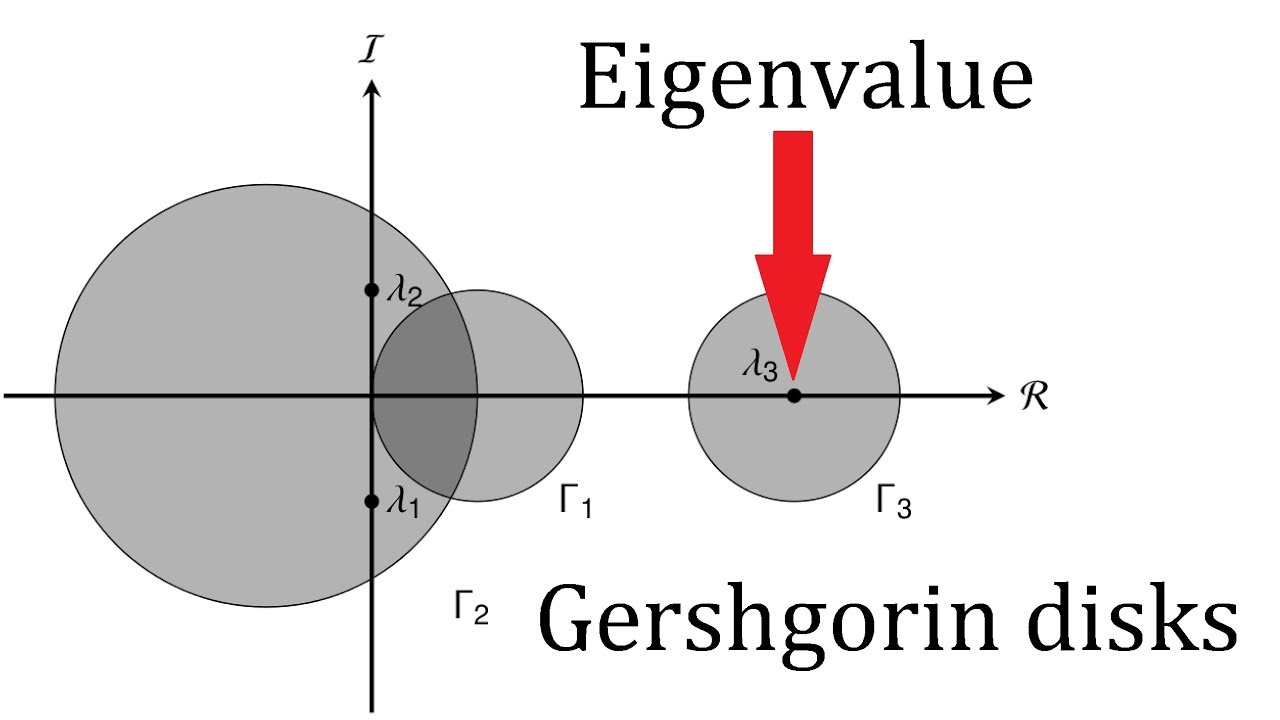
\includegraphics[width=0.45\textwidth]{pic/gresh.jpg}
		\caption{Gershgorin Circle Theorem}
	\end{figure}
\end{frame}


\begin{frame}
	\begin{itemize}
		\item Most papers and our main reference assume \(\|x_i\|=1\) and \(|y_i|\leq 1\), for simplicity.
		\item The diagonal \(H^\infty_{ii} = \frac{1}{2}\).
		\item Denote \(\rho = \max_{i,j\neq i} |x_i^\top x_j| \). Considering \(ft(t)=\frac{t(\pi-\arccos(t))}{2\pi}\), we get:
		\[
		H^\infty_{i,j\neq i} \leq \frac{\rho(\pi-\arccos(\rho))}{2\pi} \leq \frac{1}{2}
		\]
		\item We find the \textbf{Gershgorin circle} theorem and get
		\[
		 \lambda_{\min}(H^\infty) \geq  \frac{1}{2} - (n-1)\frac{\rho(\pi-\arccos(\rho))}{2\pi}
		\]
	\end{itemize}
	\begin{figure}
		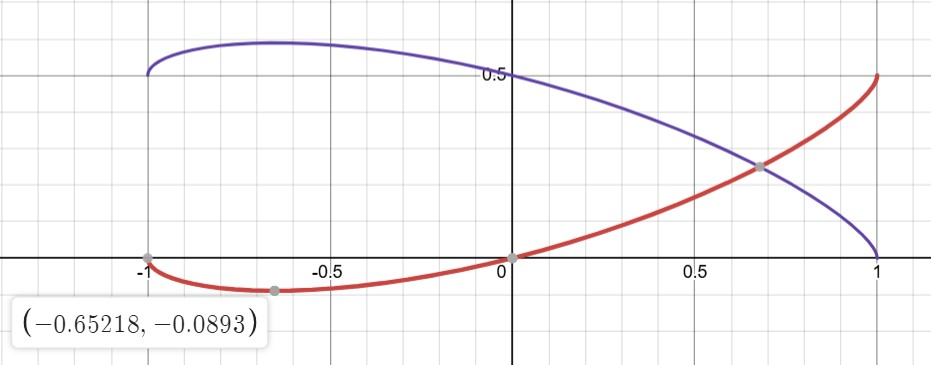
\includegraphics[width=0.7\textwidth]{pic/Arc-Cos-Func.jpg}
	\end{figure}
\end{frame}



\begin{frame}{Examples}
	\begin{itemize}
		
		\item Thus, the bound depends on the maximum "correlation" between two distinct i.i.d \(x_i\) in a sample of size \(n\). This will depend on the distribution of \(x\) on \(S^{d-1}\).
		\item The problem is now bounding \(\rho\) such that:
		
		\item \(x_i \sim \text{Unif}(S^{d-1})\):
		\[
		\max_{1 \le i < j \le n}
		\Bigl|\langle X_i,\;X_j\rangle\Bigr|
		\;\;\le\;
		C\,
		\sqrt{\frac{\log\!\bigl(\tfrac{n}{\delta}\bigr)}{d}}
		\,
		\]
		
		\item \(x_i\) are isotropic, mean-zero, sub-Gaussian vectors:
		\[
		\max_{1 \le i < j \le n}
		\bigl|\langle X_i,\;X_j\rangle\bigr|
		\;\;\le\;
		C\,
		\sqrt{\frac{\log\!\bigl(\tfrac{n}{\delta}\bigr)}{d}}
		\;\;\max_{1\le i\le n}\|X_i\|\ .
		\]
	\end{itemize}
\end{frame}

\begin{frame}{Learnable Distributions}
	\begin{itemize}
		\item \(\mathbf{y}\) has sub-Gaussian Coordinates and \(\E[y_i^2] = 2C^2\)
		\item So w.h.p. \(\|y\|_2 \leq C\sqrt{n}\)
		\item We need \(\lambda_0 \|y\|_2 \leq Cn\), so we want:
		\[
		\lambda_0 \leq C\sqrt{n} \implies  \frac{1}{2} - (n-1)\frac{\rho(\pi-\arccos(\rho))}{2\pi} \geq \frac{1}{C\sqrt{n}}
		\]
		\item For \(0 \leq \rho \leq 1\) gives a computable bound. approximately \(O(\frac{1}{n})\).
		\item So we need distributions on \(x_i\) such that \(\sup_{i,j}|\langle x_i, x_j \rangle| = O(\frac{1}{n})\) for \(n\) i.i.d samples w.h.p.
	\end{itemize}
\end{frame}


%\begin{frame}
%
%stimates from Data and Theorem Application}
%extbf{Useful Estimates:}
% from the assumptions that we have \( \| x_i \|^2_2 = \Theta(d) \) for all \( i \in [N] \) with probability \( 1 \geq N e^{-\Omega(d)} \).
%tinuity:} \( \| x_i - x_j \|^2 \leq t = dN^{-1/(r-0.5)} \), where \( t \) is the bound for \( |x_i - x_j| \).
% x_i - x_j \|^2_2 = \Theta(d) \quad \forall i \in [N], \quad |x_i - x_j|^{r} \leq dN^{-1/(r-0.5)} \quad \forall i \neq j.
%
%\frametitle{Matrix Analysis}
%ion:}
%\circ G(l+1) \circ G(l+2) \circ \dots \circ G(L).
%sitive semidefinite.
%^{L} \lambda_{\min}( G(l) ) \min_{i \in [N]} \left( \prod_{p=l+1}^L (G(p))_{ii} \right)
%_{\min}( G(2) ) = \lambda_{\min}( D \left[ \sigma(X^T w) \circ ( X^T w )^T D \right] )
%fty} \mu_s(\sigma) (X^T X^*) \right] )
%cm}
%lusion:}
%G(2) ) \geq \mu(\sigma) \lambda_{\min}( D(X^*)^T (X^*)^T D )
%a_{\min} \left( G(2) \right) \geq \lambda_{\min} \left( \sum_{i \in [N]} \| x_i \|^2_2 (X^* X^T) \right)
%\(x_i\) are almost orthogonal with high probability.
%
%\item Intuitively, we need \(x_i\) to lie on a manifold in \(\mathbb{R}^n\) such that they are distributed on it with low correlation. The data are sufficiently “spread out” in that manifold.
%	\end{itemize}
%\end{frame}
%

\begin{frame}{Weyl's Inequality}
    \textbf{Weyl's Inequality} provides bounds on the eigenvalues of the sum of two Hermitian matrices.

    \vspace{0.5cm}
    
    \textbf{Statement:} Let \( A \) and \( B \) be \( n \times n \) Hermitian matrices with eigenvalues \( \lambda_1 \leq \dots \leq \lambda_n \) for \( A \) and \( \mu_1 \leq \dots \leq \mu_n \) for \( B \). Then the eigenvalues \( \nu_i \) of the matrix \( A + B \) satisfy:
    \[
    \lambda_i + \mu_j \leq \nu_{i+j-1} \leq \lambda_i + \mu_j \quad \text{for all} \quad 1 \leq i,j \leq n.
    \]
\end{frame}

\begin{frame}
	Define:
	\begin{align*}
		A = H - \mathbb{E}[H] 
	\end{align*}
	\begin{itemize}
		\item Note that it can be shown that:
		\begin{align*}
			\mathbb{E}[H] = (\frac{1}{2} -s_d) \mathbf{1} + s_d J
		\end{align*}
		and hence \( \lambda_{\min}(\mathbb{E}[H]) = \frac{1}{2} - s_d \).
		\item Now we can take adventage of Weyl's inequality to bound the smallest eigenvalue of \(H^\infty\) via:
			\begin{align*}
				\lambda_{\min}(H^\infty) \geq \lambda_{\min}(A) + \lambda_{\min}(\mathbb{E}[H]) = \lambda_{\min}(A) + \frac{1}{2} - s_d
			\end{align*}
	\end{itemize}
\end{frame}

\begin{frame}{Main Observations}
	\begin{itemize}

		\item 	Let \( \mathbb{P} \left[ \lvert H - \mathbb{E}[H] \rvert_{op} \geq t \right] \leq \delta_t \). Then, with probability at least \( 1 - \delta_t \), we have:
		\begin{align*}
			\lambda_{\min}(H^\infty) \geq -t + \frac{1}{2} - s_d
		\end{align*}
		or equivalently:
		\begin{align*}
			\lambda_{\min}(H^\infty) \geq max \left\{ -t + \frac{1}{2} - s_d, 0 \right\}
		\end{align*}
		\item We know that \( \lvert H - \mathbb{E}[H] \rvert_{op} \) grows linearly with \( N \). Hence we can make a simple observation that one should have $O(d)$ samples to have a non-zero lower bound on the smallest eigenvalue of \(H^\infty\).
	\end{itemize}


	
\end{frame}



\begin{frame}{Future Directions \& Other Ideas}
	
\end{frame}

%%-------------------------------------------------
%\begin{frame}{Advanced Implications}
%	\begin{itemize}
%		\item \textbf{Phase Transitions}: \(\exists\) critical widths where NTK/feature learning dominates
%		\item \textbf{Quantum Analog}: NTK \(\leftrightarrow\) quantum metric tensor (geometry of NN L2 space)
%		\item \textbf{Diffusion Approx}: SGD noise \(\propto \Theta_\infty^{-1}\) (implicit regularization)
%	\end{itemize}
%	
%	\vspace{1em}
%	\textbf{Open Problems}:
%	\begin{itemize}
%		\item NTK for \textbf{dynamical} architectures (RNNs, SSMs)
%		\item \textbf{Non-Gaussian} initialization limits
%	\end{itemize}
%\end{frame}

%-------------------------------------------------


\section{References}




%\begin{frame}{Contributions}
%\textbf{These slides are authored by:}
%    \begin{itemize}
%        \item Hooman Zolfaghari
%    \end{itemize}
%    
%\end{frame}


% \begin{frame}[allowframebreaks]
%    \bibliographystyle{ieeetr} % Place the style before bibliography
%    \bibliography{ref.bib} % Point to your .bib file
%    \nocite{*} % Include all references even if not cited
% \end{frame}


\end{document}